%This is a comment

%each slide is defined with \begin{frame}{SLIDETITLE} ... \end{frame}
%1 st slide
\begin{frame}{Transfer Learning and Domain adaption}
Problems
\begin{itemize}
  \item Changes
  \begin{itemize} % itemize environments can be layered
    \item in input value(domain adaption,concept drifting)
    \item in objective of task
  \end{itemize}
  \item few examples are labelled
\end{itemize}
\end{frame}

%2 nd slide
\begin{frame}{Transfer Learning and Domain adaption}
The Definition of transfer learning
\begin{itemize}
  \item refer to the situation where what has been learned in one situation in exploited to improve $\bm{generalization} $ in another situation.
    \begin{itemize} % itemize environments can be layered
    \item So called $\bm{Inductive}$ $\bm{Transfer}$
    \item $\bm{Multi-task}$ $\bm{learning}$ involved
  \end{itemize}

\end{itemize}
\end{frame}

%3 rd slide
\begin{frame}{Transfer Learning and Domain adaption}
Shared Layer in Multi-task Learning
\begin{itemize}
\item Supervised Learning
\end{itemize}
\begin{figure}[htbp]
\centering
\begin{minipage}[t]{0.3\textwidth}
\centering
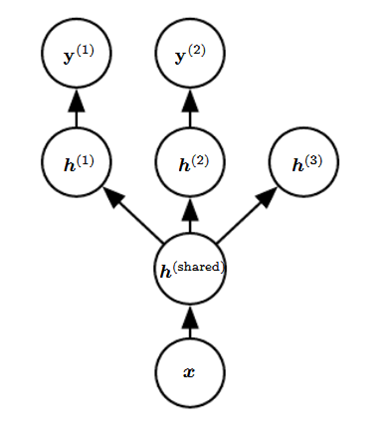
\includegraphics[width=1.2\textwidth]{Figure7_2.png}
\caption{7.2.Among semantics of input}
\end{minipage}
\begin{minipage}[t]{0.3\textwidth}
\centering
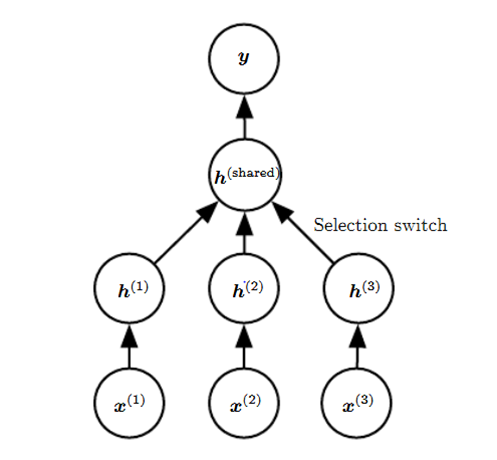
\includegraphics[width=1.4\textwidth]{Figure15_2.png}
\caption{15.2.Among semantics of output}
\end{minipage}
\end{figure}
\end{frame}

%4 rd slide
\begin{frame}{Transfer Learning and Domain adaption}
One-shot Learning
\begin{itemize}
  \item Only one(few) labeled example of the transfer task is given for one-shot learning
  \item Extract general knowledge from previously learned categories and represent it in the form of a prior probability density function in the space of model parameter
\end{itemize}
Solution[Fei-Fei et al, 2006]
\begin{enumerate} %similar to itemize but with numbers as bullets
  \item Obtain a posterior distribution
  \item Using  Conjugate Densities
  \begin{itemize} % itemize environments can be layered
    \item a conjugate prior for a given probabilistic model is one for which the resulting posterior has the same functional form as the prior
   \end{itemize}
\end{enumerate}
\end{frame}

%5 rd slide
\begin{frame}{Transfer Learning and Domain adaption}
Zero-shot Learning
\begin{itemize}
  \item No labeled example of the transfer task
  \item So called zero-data learning
   \begin{itemize}
   \item An example: consider the problem of having a large collection of text and then solve recognition problem.
   \item x: a collection of images.
   \item y: 1 - yes ; 0 - No.
   \item T: Is there a cat in this image?
   \item Text: "cats have 4 legs" or "cats have whiskers"
   \item The model is trained to estimate the conditional distribution p (y | x, T) where T is a description of the task we wish the model to perform.
   \end{itemize}
\end{itemize}
\end{frame}

%6 rd slide
\begin{frame}{Transfer Learning and Domain adaption}
Zero-shot Learning
\begin{itemize}
   \item An example: Machine Translation
   \item The model is trained to translate word A in language X to word B in language Y.
\end{itemize}
\begin{figure}[t]
\centering
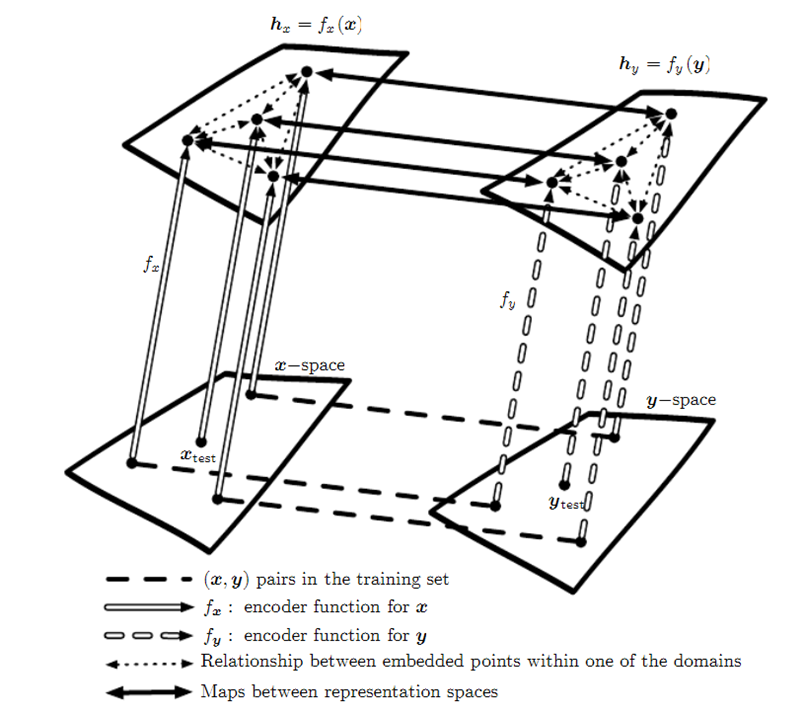
\includegraphics[width=0.4\textwidth]{Figure15_3.png} %the test_imgae is located in the "figures" folder. Place your figures there as well!
\caption{15.3.Transfer Learning between two dimension x and y enables zero-shot learning}
\end{figure}
\end{frame}

%7 rd slide
\begin{frame}{Semi-supervised Disentangling of Causal Factors}
\begin{itemize}
  \item What makes one representation better than another ?
  \item Hypothesis is that an $\bm{ideal}$ $\bm{representation}$ is one in which:
   \begin{enumerate} %similar to itemize but with numbers as bullets
   \item features are correspond to the underlying causes of the observed data.
   \item different features are correspond to different causes.
   \end{enumerate}
  \item Example: facial expression recognition
\end{itemize}
\end{frame}

%8 rd slide
\begin{frame}{Semi-supervised Disentangling of Causal Factors}
Probabilistic Model
\begin{itemize}
  \item x: observed data.
  \item y: is one of the causal factors of x.
  \item h: The representation represents all those factors.
  \item The generative process: $ p(h,x) = p(x|h)p(h) $
  \item The Marginal probability: $ p(x) = \sum\limits_{h} p(x|h) $
  \item If y are among the most salient causes, then it is easy to predict y from h.
  \item Example: David take an umbrella.
\end{itemize}
\end{frame}

%9 rd slide
\begin{frame}{Semi-supervised Disentangling of Causal Factors}
Unsupervised fail to work
\begin{itemize}
  \item no help to learn p(y|x)
\end{itemize}
Semi-supervised work successfully
\begin{itemize}
  \item if:
   \begin{enumerate} %similar to itemize but with numbers as bullets
   \item P(x) reveals precisely
   \item Components are well-seperated
   \end{enumerate}
  \item then:
  \begin{itemize}
  \item A single labeled example of each class will then be enough to perfectly learn p(y|x)
\end{itemize}
\end{itemize}
\end{frame}

%10 rd slide
\begin{frame}{Semi-supervised Disentangling of Causal Factors}
Get the most salient underlying cause
\begin{itemize}
  \item Generative adversarial networks
\end{itemize}
\begin{figure}[t]
\centering
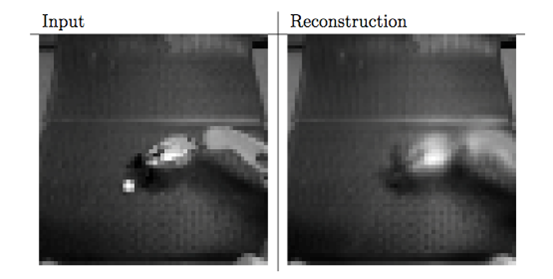
\includegraphics[width=0.8\textwidth]{Figure15_5.png} %the test_imgae is located in the "figures" folder. Place your figures there as well!
\caption{15.5. MSE vs GAN}
\end{figure}
\end{frame}

%Last slide
\begin{frame}{Semi-supervised Disentangling of Causal Factors}
Further work
\begin{itemize}
  \item Challenge 1: What to encode. More or Less ?
  \item Challenge 2: Extremely large number of underlying causes, as Brute force solution is not feasible because it is not possible to capture all the factors.
\end{itemize}
\end{frame}


